% !TeX program = pdflatex
% !TeX encoding = utf8
% !TeX spellcheck = ru_RU

\documentclass[a4paper,12pt]{SCWorks}

\usepackage{preamble}
\usepackage{minted}

\setminted{style=vs, fontsize=\small, breaklines, framesep=5mm,linenos}

\addbibresource{thesis.bib}

\begin{document}

\renewcommand{\contentsname}{Содержание}
\tableofcontents

\newpage

\section{Введение}
\label{sec:intro}

В данной работе рассматриваются математические основы и практическая реализация одного из фундаментальных методов вычислительной математики — метода Эйлера для решения обыкновенных дифференциальных уравнений. Этот метод широко используется в физике, биологии, экономике и инженерии для моделирования динамических систем~\cite{butcher2016numerical}.

На рисунке~\ref{fig:euler} представлен сам Леонард Эйлер, в честь которого назван метод.

\begin{figure}[h]
    \centering
    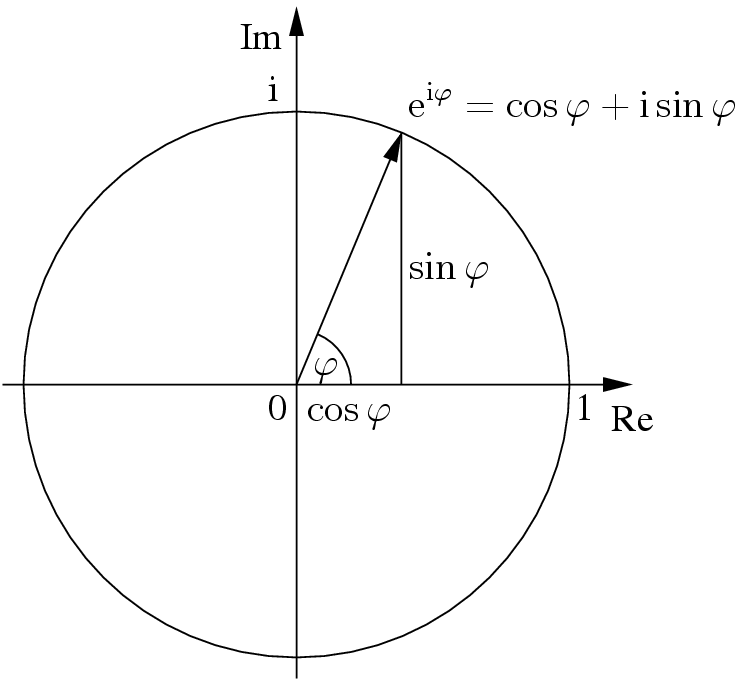
\includegraphics[width=0.4\textwidth]{images/formula.png}
    \caption{Портрет Леонарда Эйлера}
    \label{fig:euler}
\end{figure}

\section{Математическая постановка задачи}
\label{sec:math}

Рассмотрим задачу Коши для обыкновенного дифференциального уравнения первого порядка:

\begin{equation}
    \frac{dy}{dt} = f(t, y), \quad y(t_0) = y_0.
    \label{eq:cauchy}
\end{equation}

Численное решение этой задачи методом Эйлера основано на аппроксимации производной конечной разностью. Основная формула метода имеет вид:

\begin{equation}
    y_{n+1} = y_n + h \cdot f(t_n, y_n),
    \label{eq:euler}
\end{equation}

где \( h = t_{n+1} - t_n \) — шаг интегрирования. Локальная погрешность метода на одном шаге пропорциональна \( h^2 \), что можно записать как:

\begin{equation}
    \varepsilon = y(t_{n+1}) - y_{n+1} = O(h^2).
    \label{eq:error}
\end{equation}

Для иллюстрации метода рассмотрим простейшее уравнение экспоненциального роста:
\(\frac{dy}{dt} = y\) с начальным условием \(y(0)=1\). Его аналитическое решение: \(y(t)=e^t\). На рисунке~\ref{fig:plot} приведено сравнение точного решения и приближения методом Эйлера при \(h=0.5\).

\begin{figure}[h]
    \centering
    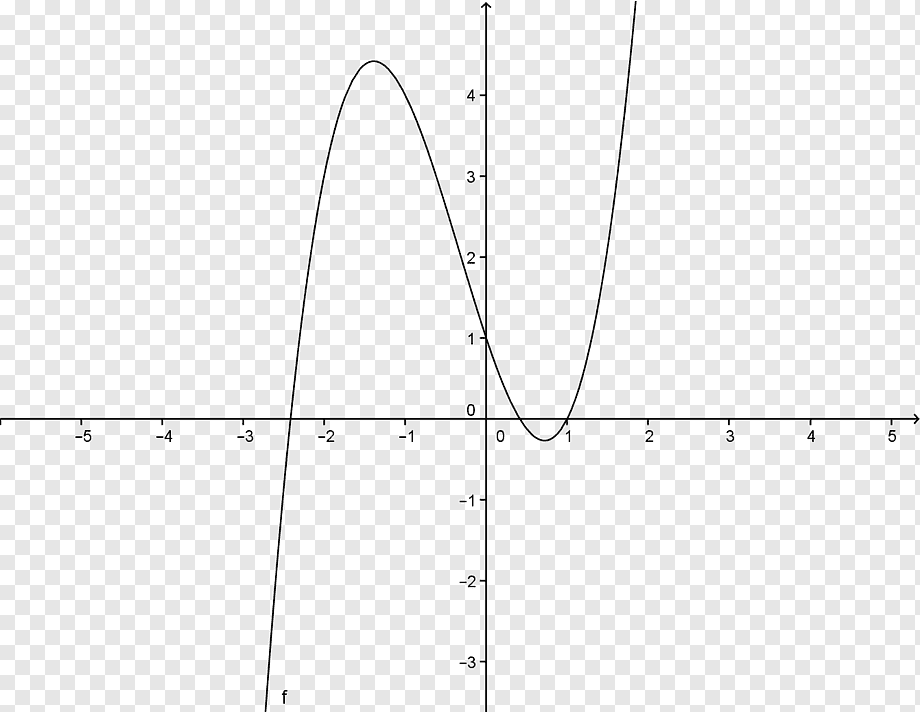
\includegraphics[width=0.7\textwidth]{images/plot.png}
    \caption{Сравнение точного решения \(y(t)=e^t\) и численного приближения методом Эйлера с шагом \(h=0.5\)}
    \label{fig:plot}
\end{figure}

\section{Программная реализация}
\label{sec:code}

Ниже представлена реализация метода Эйлера на языке Python. Функция \mintinline{python}{euler_method} принимает правую часть системы \(f\), начальные условия и шаг интегрирования, а возвращает массив точек решения.

\inputminted[firstline=5,lastline=15]{python}{code/example.py}

В этом коде переменная \mintinline{python}{h} отвечает за шаг интегрирования, а \mintinline{python}{y_values} хранит историю вычисленных значений.

\section{Численные результаты}
\label{sec:results}

В таблице~\ref{tab:results} приведены результаты вычислений для \(y' = y\) с начальным условием \(y(0) = 1\) при \(h = 0.5\).

\begin{table}[h]
    \centering
    \begin{tabular}{|c|c|c|c|}
        \hline
        \(t_n\) & Аналитическое \(y(t_n)=e^{t_n}\) & Численное \(y_n\) & Глобальная ошибка \(\delta\) \\
        \hline
        0.0 & 1.0000 & 1.0000 & 0.0000 \\
        0.5 & 1.6487 & 1.5000 & 0.1487 \\
        1.0 & 2.7183 & 2.2500 & 0.4683 \\
        1.5 & 4.4817 & 3.3750 & 1.1067 \\
        2.0 & 7.3891 & 5.0625 & 2.3266 \\
        \hline
    \end{tabular}
    \caption{Численное решение \(y' = y\) методом Эйлера с шагом \(h=0.5\)}
    \label{tab:results}
\end{table}

Как видно из таблицы, глобальная погрешность метода накапливается с каждым шагом, что согласуется с теоретической оценкой \(O(h)\).

\section{Заключение}
\label{sec:conclusion}

В рамках данной работы был рассмотрен метод Эйлера для численного решения обыкновенных дифференциальных уравнений. Были выполнены следующие задачи:
\begin{enumerate}
    \item Приведена математическая постановка задачи.
    \item Реализован алгоритм на языке Python с использованием библиотеки \mintinline{python}{numpy}.
    \item Проведены вычислительные эксперименты и выполнен анализ погрешности.
    \item Оформлен отчет в системе \LaTeX.
\end{enumerate}
Проведённое исследование подтверждает, что метод Эйлера является простым и наглядным способом численного интегрирования, но требует осторожного выбора шага для обеспечения приемлемой точности.

\section*{Список источников}
\addcontentsline{toc}{section}{Список источников}
\printbibliography[heading=none]

\end{document}